\documentclass[tikz, border=5mm]{standalone}
\usepackage{xcolor} % Required for \textcolor
\usetikzlibrary{positioning, arrows.meta, fit}

\begin{document}
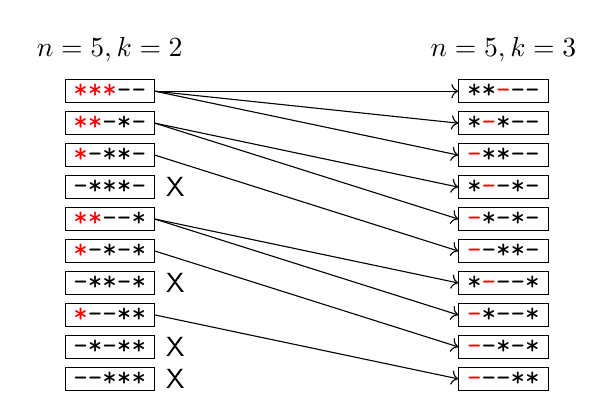
\begin{tikzpicture}[
    font=\sffamily, % Use a sans-serif font for labels
    % --- STYLES ---
    main_block/.style={black, thick, minimum width=2.5cm, minimum height=5.2cm},
    row_node/.style={
        draw,
        font=\ttfamily, % Monospaced font for symbol alignment, Large for visibility
        inner xsep=3pt,    % Padding inside row node horizontally
        inner ysep=1.5pt,  % Padding inside row node vertically
        anchor=west        % Anchor for easier alignment
    },
    x_mark/.style={font=\sffamily, text=black, inner sep=1pt},
    arrow_style/.style={->} % Arrow style
]

% --- Define content and place ROW NODES for Left Block ---
% Base position for the first row in the Left Block
\coordinate (L_start_pos) at (0, 2.5cm); % Adjust X,Y as needed for top-left of first row content

% Row 1 (L1): R B B D D
\node[row_node] (L1) at (L_start_pos) {%
    \textcolor{red}{*}\textcolor{red}{*}\textcolor{red}{*}\textcolor{black}{-}\textcolor{black}{-}%
};
% Row 2 (L2): R B D B D
\node[row_node, below=1mm of L1] (L2) {%
    \textcolor{red}{*}\textcolor{red}{*}\textcolor{black}{-}\textcolor{black}{*}\textcolor{black}{-}%
};
% Row 3 (L3): R D B B D
\node[row_node, below=1mm of L2] (L3) {%
    \textcolor{red}{*}\textcolor{black}{-}\textcolor{black}{*}\textcolor{black}{*}\textcolor{black}{-}%
};
% Row 4 (L4): D R B B D   X
\node[row_node, below=1mm of L3] (L4) {%
    \textcolor{black}{-}\textcolor{black}{*}\textcolor{black}{*}\textcolor{black}{*}\textcolor{black}{-}%
};
\node[x_mark, right=1mm of L4.east] (L4_X) {X};
% Row 5 (L5): R B D D B
\node[row_node, below=1mm of L4] (L5) {%
    \textcolor{red}{*}\textcolor{red}{*}\textcolor{black}{-}\textcolor{black}{-}\textcolor{black}{*}%
};
% Row 6 (L6): R D B D B
\node[row_node, below=1mm of L5] (L6) {%
    \textcolor{red}{*}\textcolor{black}{-}\textcolor{black}{*}\textcolor{black}{-}\textcolor{black}{*}%
};
% Row 7 (L7): D R B D B   X
\node[row_node, below=1mm of L6] (L7) {%
    \textcolor{black}{-}\textcolor{black}{*}\textcolor{black}{*}\textcolor{black}{-}\textcolor{black}{*}%
};
\node[x_mark, right=1mm of L7.east] (L7_X) {X};
% Row 8 (L8): R D D B B
\node[row_node, below=1mm of L7] (L8) {%
    \textcolor{red}{*}\textcolor{black}{-}\textcolor{black}{-}\textcolor{black}{*}\textcolor{black}{*}%
};
% Row 9 (L9): D R D B B   X
\node[row_node, below=1mm of L8] (L9) {%
    \textcolor{black}{-}\textcolor{black}{*}\textcolor{black}{-}\textcolor{black}{*}\textcolor{black}{*}%
};
\node[x_mark, right=1mm of L9.east] (L9_X) {X};
% Row 10 (L10): D D R B B   X
\node[row_node, below=1mm of L9] (L10) {%
    \textcolor{black}{-}\textcolor{black}{-}\textcolor{black}{*}\textcolor{black}{*}\textcolor{black}{*}%
};
\node[x_mark, right=1mm of L10.east] (L10_X) {X};

% We re-position L_label to be above the frame, as 'fit' might move its perceived center
\node[anchor=south, yshift=1mm] at (L1.north) {$n=5, k=2$};


% --- Define content and place ROW NODES for Right Block ---
% Base position for the first row in the Right Block
\coordinate (R_start_pos) at (5cm, 2.5cm); % Adjust X as needed

% Row 1 (R1): B B B D D
\node[row_node] (R1) at (R_start_pos) {%
    \textcolor{black}{*}\textcolor{black}{*}\textcolor{red}{-}\textcolor{black}{-}\textcolor{black}{-}%
};
% Row 2 (R2): B B D B D
\node[row_node, below=1mm of R1] (R2) {%
    \textcolor{black}{*}\textcolor{red}{-}\textcolor{black}{*}\textcolor{black}{-}\textcolor{black}{-}%
};
% Row 3 (R3): B D B B D
\node[row_node, below=1mm of R2] (R3) {%
    \textcolor{red}{-}\textcolor{black}{*}\textcolor{black}{*}\textcolor{black}{-}\textcolor{black}{-}%
};
% Row 4 (R4): B D D B B
\node[row_node, below=1mm of R3] (R4) {%
    \textcolor{black}{*}\textcolor{red}{-}\textcolor{black}{-}\textcolor{black}{*}\textcolor{black}{-}%
};
% Row 5 (R5): D B B B D
\node[row_node, below=1mm of R4] (R5) {%
    \textcolor{red}{-}\textcolor{black}{*}\textcolor{black}{-}\textcolor{black}{*}\textcolor{black}{-}%
};
% Row 6 (R6): D B B D B
\node[row_node, below=1mm of R5] (R6) {%
    \textcolor{red}{-}\textcolor{black}{-}\textcolor{black}{*}\textcolor{black}{*}\textcolor{black}{-}%
};
% Row 7 (R7): B D B D B
\node[row_node, below=1mm of R6] (R7) {%
    \textcolor{black}{*}\textcolor{red}{-}\textcolor{black}{-}\textcolor{black}{-}\textcolor{black}{*}%
};
% Row 8 (R8): B D B B B
\node[row_node, below=1mm of R7] (R8) {%
    \textcolor{red}{-}\textcolor{black}{*}\textcolor{black}{-}\textcolor{black}{-}\textcolor{black}{*}%
};
% Row 9 (R9): D D B B B
\node[row_node, below=1mm of R8] (R9) {%
    \textcolor{red}{-}\textcolor{black}{-}\textcolor{black}{*}\textcolor{black}{-}\textcolor{black}{*}%
};
% Row 10 (R10): D D B D B (Last symbol '*' in drawing)
\node[row_node, below=1mm of R9] (R10) {%
    \textcolor{red}{-}\textcolor{black}{-}\textcolor{black}{-}\textcolor{black}{*}\textcolor{black}{*}%
};

% We re-position R_label to be above the frame
\node[anchor=south, yshift=1mm] at (R1.north) {$n=5, k=3$};


% --- ARROWS ---
% Using .east and .west anchors of the row nodes
\draw[arrow_style] (L1.east) -- (R1.west);
\draw[arrow_style] (L1.east) -- (R2.west);
\draw[arrow_style] (L1.east) -- (R3.west);
\draw[arrow_style] (L2.east) -- (R4.west);
\draw[arrow_style] (L2.east) -- (R5.west);
\draw[arrow_style] (L3.east) -- (R6.west);
% L4 has X
\draw[arrow_style] (L5.east) -- (R7.west);
\draw[arrow_style] (L5.east) -- (R8.west);
\draw[arrow_style] (L6.east) -- (R9.west);
% L7 has X
\draw[arrow_style] (L8.east) -- (R10.west); % L8 -> R8
% L9 has X
% L10 has X

\end{tikzpicture}
\end{document}
